\begin{itemize}
    \item Drei Anwendungen, jeweils eine aus den Bereichen Messwerte, Nowcasting, Forecasting
    \item Messwerte: Daten Medizinmesswerte
    \item Nowcasting: Covid-Nowcasting-Hub
    \begin{itemize}
        \item Daten sind schon aufbereitet
        \item Vergleich zwischen Nowcastern möglich
        \item Noch zu klären: Wie wird $\xdiff$ gewählt?
    \end{itemize}
    \item Forecasting: Pandemie-/Epidemievorhersage, Medikamentenbedarf
\end{itemize}

\subsection{Covid nowcasting}

Data from Covid-Nowcasting-Hub


\begin{figure}
    \centering
    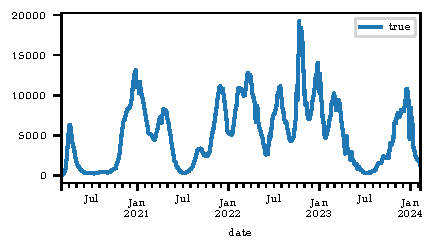
\includegraphics{plots/covid_nowcast/00_true_data.pdf}
    \caption{The seven-day-hospitalization of Covid in Germany as reported by the RKI \hl{Add citation}.}
    \label{fig:app-covid-true}
\end{figure}

\begin{figure}
    \centering
    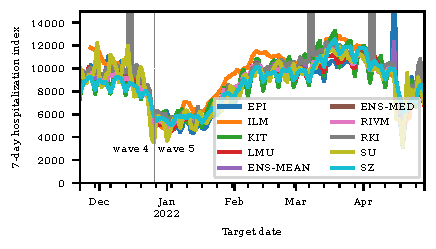
\includegraphics{plots/covid_nowcast/00_nowcast_data.pdf}
    \caption{Nowcast data without removal of outliers}
    \label{fig:app-covid-nowcast}
\end{figure}

\begin{figure}
    \centering
    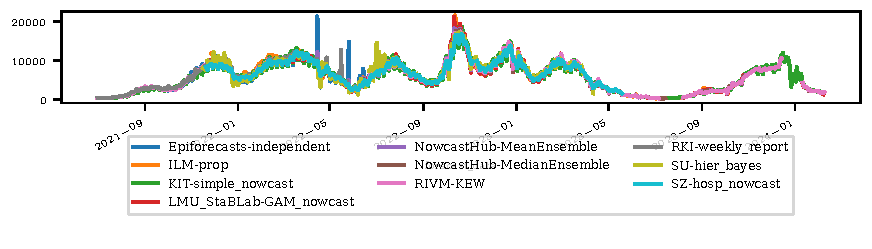
\includegraphics{plots/covid_nowcast/01_nowcast_data_without_outliers.pdf}
    \caption{Nowcast data after removal of outliers}
    \label{fig:app-covid-nowcast-no-outliers}
\end{figure}

\begin{table}[]
    \centering
    \begin{tabular}{llllr}
\toprule
 & rmse & mae & mse & count \\
model &  &  &  &  \\
\midrule
ILM-prop & :,.f & :,.f & :,.f & 530 \\
RIVM-KEW & :,.f & :,.f & :,.f & 817 \\
NowcastHub-MeanEnsemble & :,.f & :,.f & :,.f & 610 \\
NowcastHub-MedianEnsemble & :,.f & :,.f & :,.f & 610 \\
LMU_StaBLab-GAM_nowcast & :,.f & :,.f & :,.f & 574 \\
RKI-weekly_report & :,.f & :,.f & :,.f & 334 \\
KIT-simple_nowcast & :,.f & :,.f & :,.f & 861 \\
SZ-hosp_nowcast & :,.f & :,.f & :,.f & 535 \\
SU-hier_bayes & :,.f & :,.f & :,.f & 423 \\
Epiforecasts-independent & :,.f & :,.f & :,.f & 275 \\
\bottomrule
\end{tabular}

    \caption{Point evaluation measures for the issued mean of the different models. Note that not for all dates all models issue nowcasts.}
    \label{tab:app-covid-rmse}
\end{table}

\begin{itemize}
    \item Seven-day hospitalization rate as central steering measure for COVID measures in Germany
    \item Describe how it is computed
    \item Outline measures and sources to find methods
    \item Present overall measures for methods (Table~\ref{tab:app-covid-rmse})
    \item Present why trending is important, particularly the differentiation between increase and decrease
    \item Use only a subset of all methods for trending evaluation (best methods)
    \item Present trending of the subset
\end{itemize}
\subsection{Forecasting emergency department arrivals}

\textcite{Rostami-Tabar2023}

Paper setup:

\begin{itemize}
    \item (Probabilistic) forecast of the hourly number of arrivals in large emergency department (take expectation as point forecast)
    \item Forecasts are produced 48 hours ahead on a 12-hour-rolling basis; background: \enquote{It enables planners to match ED staff to the number of arrivals, redeploy staff, and reconfigure units.}
    \item training data: 2014-04-01 to 2018-2-28
    \item evaluation from 2018-03-01 to 2019-02-28
    \item Evaluation in Paper through RMSE; Pinball Loss and PIT-histograms
    \item consider several lags:
    \begin{itemize}
        \item 72-hours-lag: Is the forecast showing the correct change compared to the most recent observation (problem: strong weekly structure (i.e., Monday and Saturday highest) makes it easy to predict right direction)
        \item 7-days-lag: Correct trend compared to the last shift of same hour and day $\rightarrow$ change policies compared to that
        \item Take first issued forecast for every target time
    \end{itemize}
\end{itemize}

\begin{table}
\centering
\begin{tabular}{llll}
\toprule
 & trend acc lag 3d & trend acc lag 7d & rmse \\
\midrule
Benchmark-1 & 0.7867 & 0.7556 & 10.0654 \\
Benchmark-2 & 0.7847 & 0.7615 & 9.2462 \\
Poisson-1 & 0.7876 & 0.7661 & 9.1639 \\
Poisson-2 & 0.7886 & 0.7655 & 8.8838 \\
NOtr-1 & 0.7829 & 0.7609 & 9.4132 \\
NOtr-2 & 0.7829 & 0.7609 & 9.4132 \\
GBM-2 & 0.7697 & 0.7413 & 11.6628 \\
Ttr-2 & 0.7857 & 0.7651 & 9.3944 \\
NBI-2 & 0.7895 & 0.7656 & 8.8829 \\
qreg-1 & 0.7501 & 0.7291 & 13.3367 \\
Poisson-2-I & 0.7834 & 0.7615 & 9.4579 \\
tbats & 0.6906 & 0.6659 & 12.9049 \\
ADAM-iETSX & 0.6794 & 0.6633 & 28.0003 \\
ETS & 0.6561 & 0.6471 & 29.3577 \\
Regression-Poisson & 0.6930 & 0.6742 & 21.1623 \\
Prophet & 0.6864 & 0.6724 & 13.0785 \\
\bottomrule
\end{tabular}

\caption{Accuracies (without exclusion area) and RMSE for the considered models in \textcite{Rostami-Tabar2023}}	
\end{table}

\begin{figure}
	\centering
	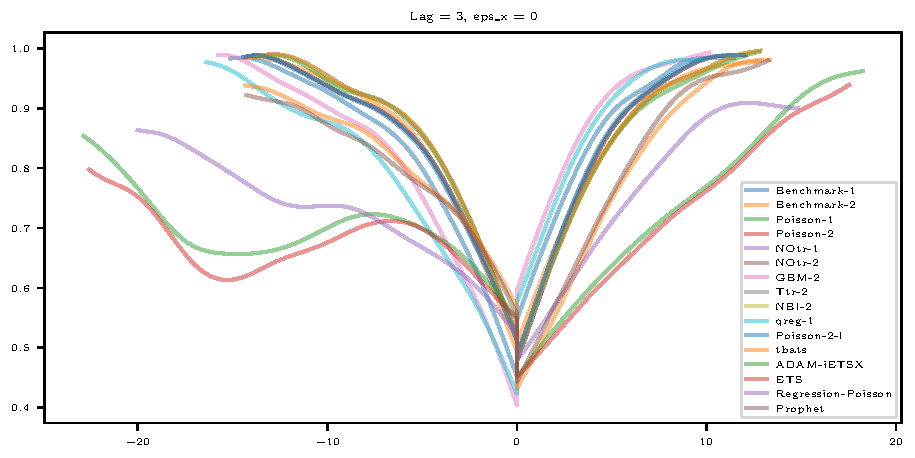
\includegraphics{plots/ed_arrival/Cond_Prob_lag_3.pdf}
        \caption{Conditional probability plot for ED arrival}
\end{figure}